\subsection{Métodos usados (UP vs. Ágil)}

UP y los métodos ágiles (como Scrum, que usamos para el primer TP) son iterativos incrementales. Sin embargo tienen varias diferencias.

UP se centra en la arquitectura, y facilita su refinamiento progresivo.

En el primer TP teníamos tres artefactos que guíaban el desarrollo de software: un Product Backlog, un Sprint Backlog y un Burndown Chart. Un backlog es simplemente una lista de prioridad de cosas a hacer. El Burndown Chart sirve para graficar el progreso durante la iteración actual. Estas tres herramientas son lo que se usa para planificar y hacer el seguimiento del proyecto en Scrum.

UP, por otro lado, contiene una larga lista de documentos y herramientas para planificar el proyecto. Por ejemplo, una planificación de una iteración de UP es muchísimo más detallada que para Scrum, dado que incluye riesgos, tareas, recursos asignados a tareas y dependencias entre tareas.


\begin{figure}[H]
  \centering
  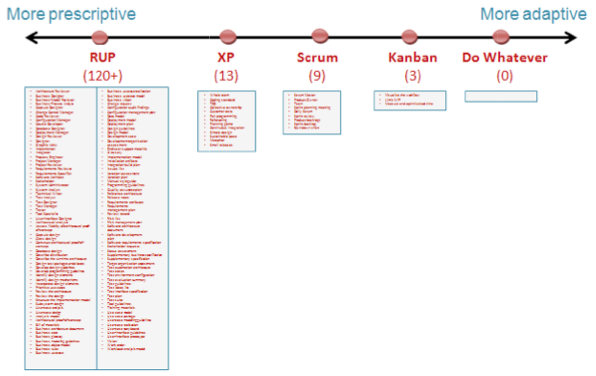
\includegraphics[width=0.7\textwidth]{img/up-agile.png}
  \caption{\normalfont Comparación de varias metodologías de desarrollo.}
\end{figure} 

\subsection{Programming in the small y Programming in the large}

Programming in the large y programming in the small describen dos aproximaciones diferentes al diseño y desarrollo de software. 

Programming in the large involucra en general productos de software desarrolloados por grupos a lo largo de extensas cantidades de tiempo. Con programming in the large, los diseñadores hacen hincapié en particionar el trabajo en modulos con interacciones bien definidas. Esto requiere una cuidadosa planificación además de una cuidadosa documentación. Programming in the large en general se refiere a diseñar el sistema desde un alto nivel, donde solo importa el estado de los módulos y sus interacciones, y no su implementación real.

Debido a todas estas características, el programming in the large es importante planificar a largo plazo, tener en cuenta riesgos y darle mucha importancia a la arquitectura del software. Por esta razón, programming in the large suele estar asociado con UP.

Por otro lado, programming in the small describe la actividad de escribir pequeños programas, es decir, cuyo desarrollo toma poco tiempo. En general programming in the small es llevado a cabo por personas individuales o pequeños equipos.

Debido a que en general se busca velocidad en el desarrollo de estas pequeñas piezas de software, y mejorarlas de manera incremental, programming in the small suele asociarse con métodos de desarrollo ágiles, como Scrum.

\subsection{Conclusiones generales}

???
